\section{Experimental Evaluation}

\begin{figure}
  \lstset{language=C, basicstyle=\small}
  \begin{lstlisting}
#define N 200

int main(void){
  int value = 0xCafeBabe;
  int *buffer;
  int i = 0;

  buffer = (int*)malloc(N*N*sizeof(int));

  for ( i = 0 ; i < N*N ; i++ ) {
      buffer[i] = value;
  }

  return buffer[0];
}
  \end{lstlisting}
  \caption{The source code for \texttt{test\_init} program. (Note the memory leak is intentionally.)}
  \label{fig:test_init}
\end{figure}

As one of our goals was to provide a fast replay mechanism for the
logged data. We developed, based on the cache simulator from our
$1^{st}$ assignment (furthermore referred as \emph{scs\_pin}), a cache
simulator that uses our replay mechanism (furthermore referred to as
\emph{scs\_replay}). Given the fact, that our pin version of the cache
simulator already used the Executor abstraction, the port was straight
forward and allowed us to compare functionally and implementation wise
completely identically cache simulators with each other. To evaluate
the performance we wrote a simple benchmark program (see Figure
\ref{fig:test_init}) that initialize a memory array. We then evaluated
and compared the two following approaches by varying the parameter N:

\begin{description}
  \item[scs\_pin] Run the benchmark application with the pin version of
    our cache simulator.
  \item[scs\_replay] First run the benchmark application with our pin
    tool to gather a trace file. Then we used this trace file as
    source for our replay library.
\end{description}

\begin{table*}
  \begin{tabularx}{\textwidth}{X r r r r r}
    \toprule
    Program/Configuration & Time (no logging) [s] & Time (logging) [s] & log size [bytes] & scs\_relay [s] & scs\_pin [s]\\
    \midrule
    %% helloword         & 1.21 & 12.14 &  6961152 & 0.70  & 0.89 \\
    \addlinespace[1mm]
    \rowcolor[gray]{.9}
    text\_init/N=10   & 1.23 & 11.48 &  6601728 & 0.66 & 0.89 \\
    \addlinespace[1mm]
    text\_init/N=20   & 1.23 & 11.48 &  6717440 & 0.66 & 0.89 \\ 
    \addlinespace[1mm]
    \rowcolor[gray]{.9}
    text\_init/N=30   & 1.25 & 12.07 &  6912000 & 0.70 & 0.90 \\
    \addlinespace[1mm]
    text\_init/N=40   & 1.24 & 12.57 &  7183360 & 0.74 & 0.90 \\
    \addlinespace[1mm]
    \rowcolor[gray]{.9}
    text\_init/N=50   & 1.25 & 13.19 &  7532544 & 0.76 & 0.90 \\
    \addlinespace[1mm]
    text\_init/N=100  & 1.24 & 18.71 & 10441728 & 1.08 & 0.90 \\
    \addlinespace[1mm]
    \rowcolor[gray]{.9}
    text\_init/N=150  & 1.26 & 27.79 & 15292416 & 1.60 & 0.90 \\
    \addlinespace[1mm]
    text\_init/N=200  & 1.28 & 40.57 & 22071296 & 2.33 & 1.04 \\
    \bottomrule
  \end{tabularx}
  \caption{Performance evaluation and comparison of between the cache
    simulator using directly the pin infrastructure and using out
    replay library.}
  \label{tbl:results}
\end{table*}

Table \ref{tbl:results} summaries the results we got from our
evaluation. Note that there is a change of the stepping. While the
first 4 runs increase N by 10, the last 4 runs increased N by 50. The
following section will discuss these results in more details.

\begin{figure}
  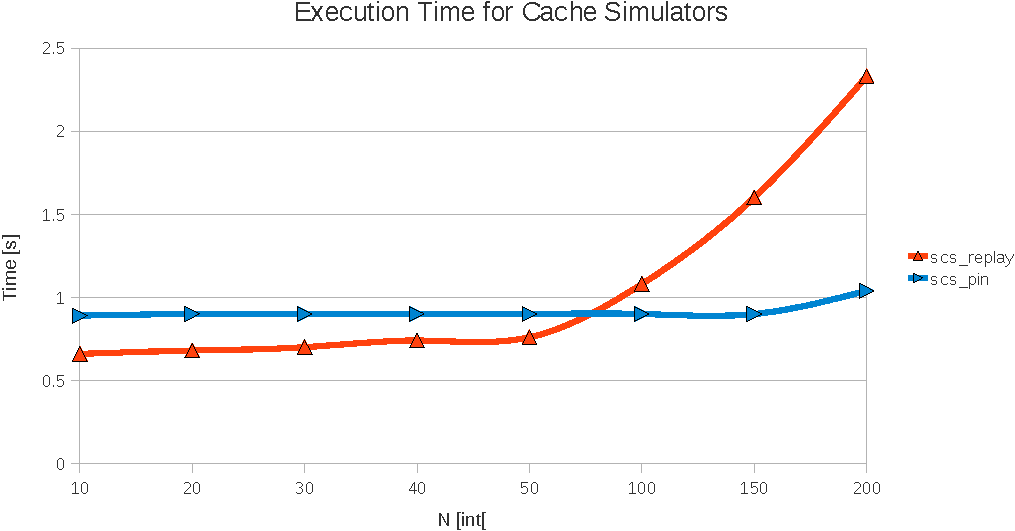
\includegraphics[width=\columnwidth]{eval_execution_time_replay}
  \caption{The execution time of the cache simulator using the pin
    infrastructure or our replay library.}
  \label{fig:eval_execution_time_replay}
\end{figure}

As our main goals was to provide a faster way of performing analysis,
our main interest was the comparison of the cache simulator execution
times. As shown in Figure \ref{fig:eval_execution_time_replay} is the
execution time for the replay version only for very small N better
than for the `native' pin tool version. As soon as N gets bigger than
100, we can see a clear trend towards a drastic performance penalty
for our replay approach. In the next section we will break down our
analysis of this phenom.

\begin{figure}
  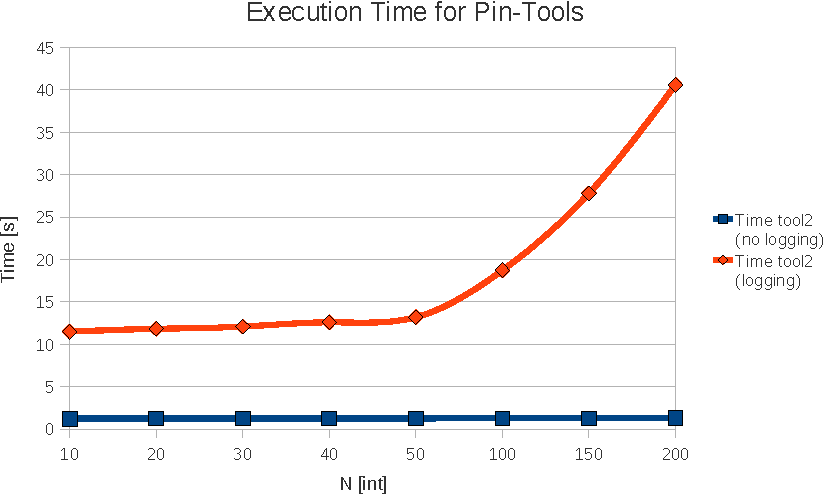
\includegraphics[width=\columnwidth]{eval_execution_time_tracing}
  \caption{The execution time of our tracing generator, comparing the
    case where actual data is written and the case where we just run
    the application without performing any log operation.}
  \label{fig:eval_execution_time_tracing}
\end{figure}

\begin{figure}
  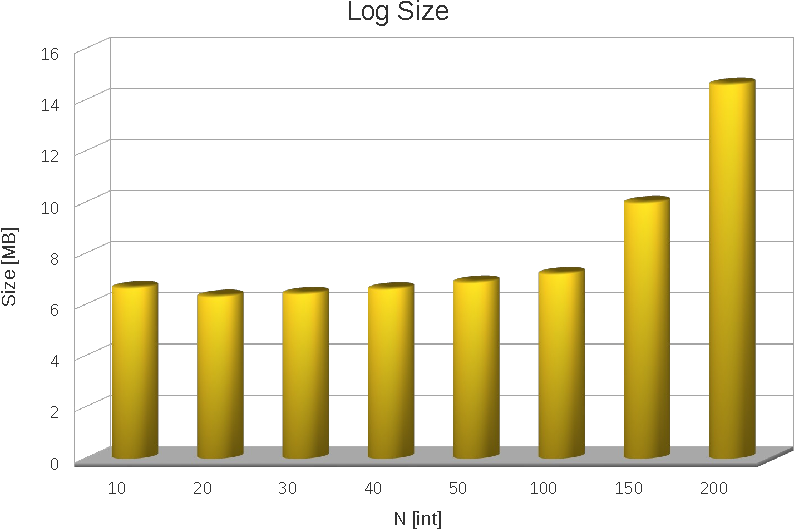
\includegraphics[width=\columnwidth]{eval_log_size}
  \caption{The evaluation of the log size while changing parameter N of the \texttt{test\_init} program. }
  \label{fig:eval_log_size}
\end{figure}


While gathering the tracing information we already realized a
performance hit. To get an better understanding of the possible
performance costs of the SQLite database we compared the dry-run mode
of our pin tool, which does not write any logging information, with
the normal mode of our pin tool. The results are shown Figure
\ref{fig:eval_execution_time_tracing}. As can clearly shown by the
execution time for the case without writing any logging information
performs almost linear, while execution with writing logging
information at least one order of magnitude worse (with a clear trend
to become exponential). A reason for this behavior can directly be
inferred when observing the amount of data that is stored in the
database, as shown in Figure \ref{fig:eval_log_size}\footnote{Note
  that the store operations modify a database table and not just
  append the file.}. To second our observation and evaluate if there
is a single root cause, the we could potentially overcome, recompiled
the whole software stack with profiling information and re-run the
replay cache simulator with the input for N = 200. As shown in the
Figure \ref{fig:profiler}, almost half of the time is just wasted by
an internal SQLite function, converting the data from the database
into a sting representation.


\begin{figure}
  \lstset{language=C, basicstyle=\small}
  \begin{lstlisting}
int main(void) 
{
  int *result = (int*)malloc(sizeof(int));
  int value = 3;
  
#pragma omp parallel for 
  for ( int i = 0 ; i < 100  ; i++ )  {
    if ( i % value == 0) {
      #pragma omp critical 
      {
        if ( *result < i ) {
          *result = i;
        }
      }
    }
  }
}
  \end{lstlisting}
  \caption{The source code for \texttt{test\_openmp} program.}
  \label{fig:test_openmp}
\end{figure}



Compare with FDR, which claims 2\% slowdown in a typically scenario
and 34 MB log files (for 1 billion instruction replay window)
per processor in addition to a full memory dump.

Compare with BugNet, whose First Load Log grew to ~100 MB in the worst
case and less than 20 MB on average when using a window of 1
billion instructions.

Compare with Eraser.  Programs run 10 to 30 times slower with Eraser.

SIGMA does not report slowdown caused by instrumentation, but shows
that some of its logs can grow to hundreds of MB even \emph{after} compression.
However, in other cases a several hundred MB trace is compressed
to a less than 1 MB trace.

MemSpy results in 22 to 58 times slowdown during testing on a single processor.

\begin{figure*}
  \lstset{basicstyle=\footnotesize, mathescape=true}
  \begin{lstlisting}
Each sample counts as 0.01 seconds.
  %   cumulative   self              self     total           
 time   seconds   seconds    calls  ms/call  ms/call  name    
 43.44      0.43     0.43  4047013     0.00     0.00  sqlite3VXPrintf
 12.12      0.55     0.12   809419     0.00     0.00  sqlite3VdbeExec
  6.06      0.61     0.06   758517     0.00     0.00  Profiler::addToRead(long, long, long, long)
  3.03      0.64     0.03  5665887     0.00     0.00  sqlite3ApiExit
  3.03      0.67     0.03  4047031     0.00     0.00  sqlite3ValueText
  3.03      0.70     0.03  4047017     0.00     0.00  sqlite3StrAccumAppend
  3.03      0.73     0.03   809305     0.00     0.00  Profiler::addToUsage(long, long)
  2.53      0.76     0.03  4047023     0.00     0.00  sqlite3VdbeSerialGet
  2.02      0.78     0.02  4047031     0.00     0.00  sqlite3VdbeChangeEncoding
  2.02      0.80     0.02  4047023     0.00     0.00  columnMem
  2.02      0.82     0.02  4047012     0.00     0.00  sqlite3_snprintf
  2.02      0.84     0.02   809401     0.00     0.00  callback(void*, int, char**, char**)
  1.52      0.85     0.02  4047059     0.00     0.00  sqlite3DbMallocSize
  $\vdots$
  \end{lstlisting}
  \caption{GProf results of the cache simulator run using our replay library}
  \label{fig:profiler}
\end{figure*}
